\documentclass[a4paper,10pt,twoside]{book}

\usepackage{graphicx}
\usepackage[normalem]{ulem}

\newcommand{\ct}[1]}
\usepackage{listings}

\lstnewenvironment{code}[1]{%
	\lstset{%
		% frame=lines,
		frame=single,
		framerule=0pt,
		mathescape=false
	}
}{}

\lstnewenvironment{script}[2][defaultlabel]{%
\renewcommand{\lstlistingname}{Script}%
	\lstset{
		% frame=lines,
		frame=single,
		framerule=0pt,
		mathescape=false,
		name={Script},
		caption={\emph{#2}},
		label={scr:#1}
	}
}{}
\usepackage{fixltx2e}
\usepackage[
	colorlinks=true,
	linkcolor=black,
	urlcolor=black,
	citecolor=black
]{hyperref}

\begin{document}

\chapter{Introduction}
Have you ever wanted to develop advanced client side applications without having to deal with the asynchronous 
nature of Javascript? Wouldn't you love to share your models between your client and your server? Then Tide
is made for you. Tide is a client-side web framework developed in Pharo and Amber. \href{https://github.com/tide-framework/tide}{Tide} offers seamless communications between \href{http://amber-lang.net}{Amber} and  \href{http://pharo-project.org}{Pharo}.

An application developed in Tide is composed of two parts: one part in Pharo to define what we call a presenter model and one part in Amber for the client-side widgets. Tide ensures the communication between these two parts Tide exchanges information using the \ct{JSON} format. The \ct{JSON} is built from  Pharo objects and sent through the network to Amber.Having both data and actions sent to Amber makes Tide a very good communication protocol between the client and server.

But there is something fundamentally different in Tide: The \ct{JSON} contains data exposed from objects in Pharo, but it also contains callback information to perform actions from Amber to Pharo objects. Let us look at the implications raised. Generating JSON is trivial and used more and more as a way to replace XML. However, having operations (callbacks) describing how to interact with data is a key difference: It lets you factor out the logic of your application. You do not get just data and are forced to 
recreate on the client-side some logic. You get fully described data, therefore it is easier to build generic and reusable client-side widgets manipulating data. 

This documentation will teach how to install and use Tide through examples.  
We will also learn its architecture and more advanced topics.

SD: What we will learn concretely.
\chapter{ Installing Tide}\section{ Prerequisites}
Tide requires several libraries. It of course depends on Pharo and Amber. Amber
itself requires \ct{nodejs} and \ct{bower} to install its own dependencies. The 
Pharo-side of Tide requires Zinc, which is part of the default image since 
Pharo 2.0. Tide however has only been tested with Pharo 3.0.
\subsection{ NodeJs}
Go to \href{http://nodejs.org}{nodejs.org} and install \ct{node} (and \ct{npm}) for your
platform.
\subsection{ Bower}
Bower is a package manager for the web, and Amber uses Bower to manage 
dependencies. The simplest way to use bower is to install it globally as 
follows:


\begin{code}{}
$ npm install -g bower
\end{code}

\subsection{ Pharo}
Tide requires Pharo 3.0. The simplest way to install it is to evaluate the 
following:


\begin{code}{}
$ curl get.pharo.org/30+vm | bash
\end{code}


To start the Pharo image, evaluate:


\begin{code}{}
$ ./pharo-ui Pharo.image
\end{code}

\subsubsection{ Preparing the Pharo image}
SD: We can also do it from the command line and it would be good to show how. 
SD:Would be good to have one release of tide 
to avoid development. 

Once you get the Pharo window open, you have to install the Tide backend part. 
This means bringing the Pharo code you cloned from GitHub?? into the Pharo image.

\begin{itemize}
\item  Click on the background of the Pharo window
\item  In the World menu that appears, click on \ct{Workspace}
\item  In that window, evaluate: (you type the thing, select the text and then right 
\end{itemize}

  click and select \symbol{34}Do It\symbol{34} from the menu).


\begin{code}{}
Metacello new
  configuration: 'Tide';
  version: #development;
  repository: 'http://www.smalltalkhub.com/mc/Pharo/MetaRepoForPharo30/main';
  load.
\end{code}


SD: Why the following is not in the troubleshooting session and bower install is not executed before?

When this is finished, evaluate:


\begin{code}{}
TDDispatcher tideIndexPageUrl inspect
\end{code}


When first executed, you will get an error saying you must execute bower 
install in a particular directory. Open a terminal, change to the right 
directory, and execute:


\begin{code}{}
$ bower install
\end{code}


SD: add screenshots

Back in the Pharo window, close the error message and evaluate the same instruction 
again:


\begin{code}{}
TDDispatcher tideIndexPageUrl inspect
\end{code}


This should give you the URL at which your web browser should be pointed to. 
Now copy this URL, open your web browser and paste it in the browser's address bar.

SD: why do we need to do this inspects? because it gives the impression that everything is manual?
\subsection{ Starting the server}
The \ct{TDServer} class provides a convenient way to start$/$stop a Tide server, using
Zinc behind the scenes:


\begin{code}{}
TDServer startOn: 5000. "Start the server on port 5000"
TDServer stop. "Stop any running server"
\end{code}

\chapter{ A first example: the traditional counter}
To get started with Tide, we will implement the traditional counter example as shown in Figure \ref{tideCounter}. 
Note that Tide already includes such an example in the \ct{Tide-Examples} package that you can refer to.
But better follow step by step the example.


\begin{figure}

\begin{center}
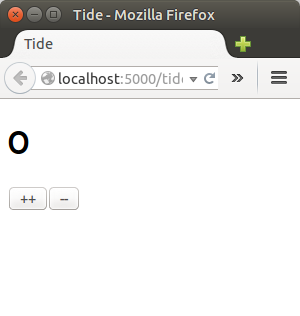
\includegraphics[width=0.6\textwidth]{images/tide-counter.png}\caption{A tide counter.\label{tideCounter}}\end{center}
\end{figure}


SD: picture should be cut in horizontal

Developing an application in Tide consists in two main elements, the presenter part developed in Pharo subclassing some Tide classes
 and the client side developed in Amber. 

A counter application should contain two buttons, one to increase and the other one to decrease a count. It should also display the count value to the user. While this application might seem extremely simplistic, it already shows some of the 
core principles behind Tide: Presenters and Proxies.
\section{ The Pharo presenter part}
We start by creating the \ct{MyCounter} class in Pharo by subclassing \ct{TDPResenter}.


\begin{code}{}
TDPresenter subclass: #MyCounter
	instanceVariableNames: 'count'
	classVariableNames: ''
	category: 'MyCounter'
\end{code}


Note that not all \symbol{34}exposed\symbol{34} objects have to be subclasses of \ct{TDPresenter}. As we will
see later, any object can be exposed to Amber using a \ct{TDModelPresenter} instance
on the domain object. SD: we should also say that latter we will explain what is a TDPresenter.

Our class has one instance variable \ct{count} that we initialize to \ct{0}:


\begin{code}{}
MyCounter >> initialize
    super initialize.
    count := 0
\end{code}


To display the count value to the user, we will need to expose \ct{count} using an accessor.
We also add two methods to increase and decrease our counter:


\begin{code}{}
MyCounter >> count
    ^ count

MyCounter >> increase
    count := count + 1

MyCounter >> decrease
    count := count - 1
\end{code}


The final step we need to add the our counter is pragmas. Pragmas are 
method metadata. Tide uses pragmas to expose data (called state in Tide) 
and callbacks (called actions) to Amber. Here's our final version of the 
counter class:


\begin{code}{}
MyCounter >> count
    <state>
    ^ count

MyCounter >> increase
    <action>
    count := count + 1

MyCounter >> increase
    <action>
    count := count - 1
\end{code}

\section{ Registering applications with handlers}
We now have to create an entry point with our counter presenter in the Tide server.
To register the entry point, evaluate:


\begin{code}{}
MyCounter registerAt: 'my-counter'.
\end{code}


If we perform a request at \ct{http:$/$$/$localhost:5000$/$my-counter}, we get the following 
\ct{JSON} data back:


\begin{code}{}
{
  "__id__":"bwv8m74bhgzmv0dgvzptuy4py",
  "actions":{
    "increase":"/my-counter?_callback=359446426",
    "decrease":"/my-counter?_callback=523483752"
  },
  "state":{
    "count":0
  }
}
\end{code}


SD: how can I for example get an inspector on the MyCounter instance to increase it. So that the developer sees it live.
\section{ Stepping back}
We can learn a couple of points from the preceding example:

\begin{itemize}
\item  Presenter classes are registered as handlers, not instances. Tide will create \symbol{34}per session\symbol{34} instances of the registered class meaning that presenters are not shared between user sessions.
\item  The entry point will have a \ct{handler} associated with a fixed entry point  url \ct{'$/$my-counter'}. When someone will query that registered url, the presenter will generate \ct{JSON} data corresponding to its state and actions, and the handler to send it back in a response to the request.
\item  Sending JSON is common and trivial using a Pharo package such as NeoJSON. What is much more interesting with Tide is the fact that exchanged data is described with the operations that can be applied to it. It provides an object-oriented view on the data. You get serialized active objects and not plain dead data.
\end{itemize}
\section{ The Amber part of the application}
The next step in our example is to create the Amber-side of this counter application.

SD: say that Amber will do it for us: 
We will use Amber to render an HTML view of our counter, and perform actions using proxies
back to the counter defined in Pharo.
\subsection{ The client-side API}
On the client-side, root presenters exposed as handler can be accessed by creating proxies:
SD: It is not clear that we have presenters on Pharo and Amber. We should explain that before section presenters.


\begin{code}{}
myProxy := TDClientProxy on: '/my-counter'.
\end{code}


Interacting with proxies is performed via messages. However we have two kinds of messages. Messages sent to proxies will be resolved using their \textbf{state} and \textbf{actions+} as defined on the server-side. SD: what is an actionplus? we did not introduce the terms like that.

\begin{itemize}
\item  Calls to state methods are resolved locally and synchronously, because the state is passed over to Amber as we previously say in the JSON data.
\end{itemize}

\begin{itemize}
\item  Calls to action methods perform requests that will result in performing the corresponding
\end{itemize}

method on the Pharo object asynchronously. Once the action is performed, the proxy will
be automatically updated with possible new state and actions.
\subsection{ Handling asynchronous calls}
Since action calls are not synchronous, Tide proxies have a special method \ct{then:} used
to perform actions only when and if the action is resolved and the proxy updated.

Sending a message that activates a state method is synchronous as shown in the following snippet.

\begin{code}{}
"synchronous state call"
myProxy count. "=> 0"
\end{code}


Now sending a message that activates a callback is asynchronous and as such we should use the \ct{then:} message when we want to access the state as shown below: 

\begin{code}{}
"async action call"
myProxy increase; then: [
    myProxy count "=> 1" ]
\end{code}


SD: the developer in Pharo could use a convention to make this explicit. Is it wise to have countState?
\subsection{ The widget class}
In Amber's IDE, create a new class \ct{MyCounterWidget}. 


\begin{code}{}
Widget subclass: #MyCounterWidget
	instanceVariableNames: 'counter header'
	package: 'Tide-Amber-Examples'
\end{code}


The widget class has two instance variables: \ct{counter}, which holds a proxy over the 
Pharo counter object, and \ct{header} which  holds a reference on the header tag brush to
update the UI.

To initialize our counter widget, we connect it to the Pharo counter presenter as follows:


\begin{code}{}
MyCounterWidget >> initialize
    super initialize.
    counter := TDClientProxy on: '/my-counter'
\end{code}


Note that \ct{'$/$my-counter'} is the path to the server-side handler for our counter presenter.

We can now create the rendering methods as follows


\begin{code}{}
MyCounterWidget >> render
    counter connect then: [
        self appendToJQuery: 'body' asJQuery ]

MyCounterWidget >> renderOn: html
	header := html h1 with: counter count asString.
	html button 
		with: '++';
		onClick: [ self increase ].
	html button 
		with: '--';
		onClick: [ self decrease ]

MyCounterWidget >> update
	header contents: [ :html |
		html with: counter count asString ]
\end{code}


The \ct{render} method waits for the counter to be connected, then appends the widget to the
\ct{body} element of the page (using the \ct{renderOn:} method).

SD: why the previous part is not in the framework. Why any user will have to define it?
SD: where is the link between appendTOJQuery and renderOn:?

  \ct{renderOn:} is a typical widget rendering method using the builtin Amber \ct{HTMLCanvas}.
The \ct{count} message send to the \ct{counter} proxy will be resolved as a state accessor as
defined on the server-side.

Finally instead of updating the entire HTML contents of the counter, \ct{update} will only 
update the relevant part, the header.

We still miss two methods to actually increase and decrease our counter:


\begin{code}{}
MyCounterWidget >> increase
	self counter increase.
	self counter then: [ self update ]

MyCounterWidget >> decrease
	self counter decrease.
	self counter then: [ self update ]
\end{code}


SD: we also miss counter. is it a method that we should define?

Here's a screenshot of the final counter application:


\begin{figure}

\begin{center}
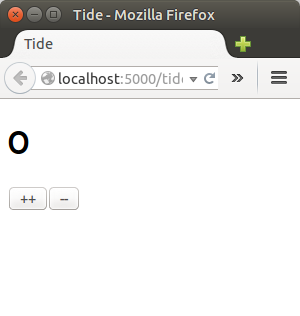
\includegraphics[width=1.0\textwidth]{images/tide-counter.png}\caption{file:$/$$/$images$/$tide-counter.png.\label{images/tide-counter.png}}\end{center}
\end{figure}

\chapter{ Actions}
We have seen in a nutshell in the previous sections how Tide actions work. They allow callbacks
to be performed from Amber to Pharo objects.

What we haven't discussed yet is how action callbacks in Tide can pass arguments to Pharo objects.
\section{ Action arguments}\subsection{ Literals}
Literal objects can be send as arguments to Tide actions. They will be converted to JSON and back in
Pharo. Any literal that can be serialized to JSON can be send as an argument:

\begin{itemize}
\item  Numbers
\item  Booleans
\item  Strings
\item  Dictionaries
\item  Arrays (and OrderedCollections)
\end{itemize}

As an example, we can improve the counter to be able to increase it by any number instead of one:


\begin{code}{}
MyCounter >> increaseBy: anInteger
    <action>
    count := count + anInteger
\end{code}


On the Amber side, we can change the \ct{increase} method to increase the counter by 8:


\begin{code}{}
MyCounterWidget >> increase
    self counter increaseBy: 8; then: [
        self update ]
\end{code}

\subsection{ References}
While sending literals from Amber to Pharo is definitely useful and convenient, it is barely enough for more
complicated scenarios, where more complex objects have to be sent as arguments.

To manage this use case, Tide allows references to presenters to be used as action arguments too. 
This means that any presenter proxy in Amber can be used as an argument to an action argument, and 
that identity will be preserved on the Pharo side when the action message will be sent.
\section{ Chaining actions}
Tide actions can be easily chained without breaking the sequential flow of the application code, 
using promises. This is an important property of action callbacks, because all requests done in 
the client must be asynchronous, quickly leading to \symbol{34}spaghetti callbacks\symbol{34} code.

SD: here we should have a JS example of async and show how we can express it in tide. 
\subsection{ Back to the counter example}
The following code snippet shows how \ct{increase} calls to our counter are chained.
SD: using \ct{then:}


\begin{code}{}
myCounter := TDClientProxy on: '/my-counter'.

myCounter increase; increase.
myCounter then: [ myCounter count ]. "=> 2"

10 timesRepeat: [ myCounter decrease ].
myCounter then: [ myCounter count ]. "=> -8"
\end{code}

\chapter{ Presenters}
Tide makes it easy to create presenters on domain objects.
\section{ Root presenters}
In any Tide application, some presenters must be always accessible at a fixed url. They are called 
in Tide terminology root presenters. Root presenters are the entry points of Tide application.

We already saw one root presenter, the \ct{MyCounter} class.

To register a presenter class, use \ct{TDPresenter$>$$>$registerAt:}. Tide will register the presenter 
class with the corresponding path and create instances per session.

Note that only one instance of registered root presenter class will be created per session. This 
ensures that all actions will be performed on the same object.
\section{ Answering new presenters from action callbacks}\subsection{ A note about security}\section{ Builtin presenter classes}\section{ Custom presenters}\section{ Presenters and security}\chapter{ Managing sessions}\chapter{ Handlers}
\begin{todo}

should it be there already? It seems too early to talk about that, but I need to introduce the concept in order to talk about the file upload handler.
\end{todo}
\chapter{ Managing file uploads}
Managing file uploads in the context of a flat-client application can be cumbersome. 
The reason is that file uploads with the HTTP protocols were not made for asynchronous 
uploads. Tide tries to solve this problem by abstracting away the implementation details 
of an AJAX-friendly file upload with the \ct{TDFileHandler} class.
\section{ Creating file upload entry points}\chapter{ Handling exceptions}\chapter{ A more advanced example: }
We should use the example of the book of Olivier: a comix collection. 


\end{document}
